\documentclass[apectratio=169]{beamer}
\usetheme{metropolis}           % Use metropolis theme
% For PDFs
\usepackage{pdfpages}
\usepackage{minted}
\usepackage{tabularx}
\title{DIY Etching Machine}
\subtitle{State of the Art (Papers) and Market Analysis}
\date{\today}
\author{Nils Weber and Maximilian Stiefel}
\institute{Uppsala University}
\begin{document}
  \maketitle

\begin{frame}{Table Of Contents}
  \setbeamertemplate{section in toc}[sections numbered]
  \tableofcontents[hideallsubsections]
\end{frame}

\section{Papers}

\begin{frame}{A buck converter controller design in an electronic drive for LED lighting applications [Iturriaga-Medina et al., 2015]}
  \begin{figure}
    \centering
    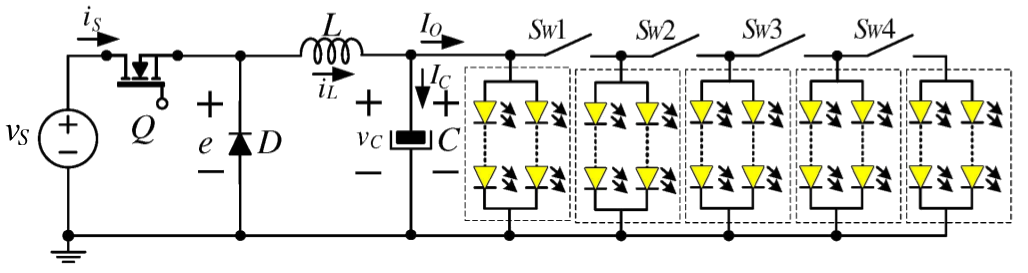
\includegraphics[scale = 0.42]{./fig/paper1}
    \caption{Bucket converters are very common in power electronics.}
  \end{figure}	
\end{frame}

\begin{frame}{High-Efficiency Resonant LED Backlight Driver with Passive Current Balancing and Dimming [Xueshan Liu et al., 2017]}
  \begin{figure}
    \centering
    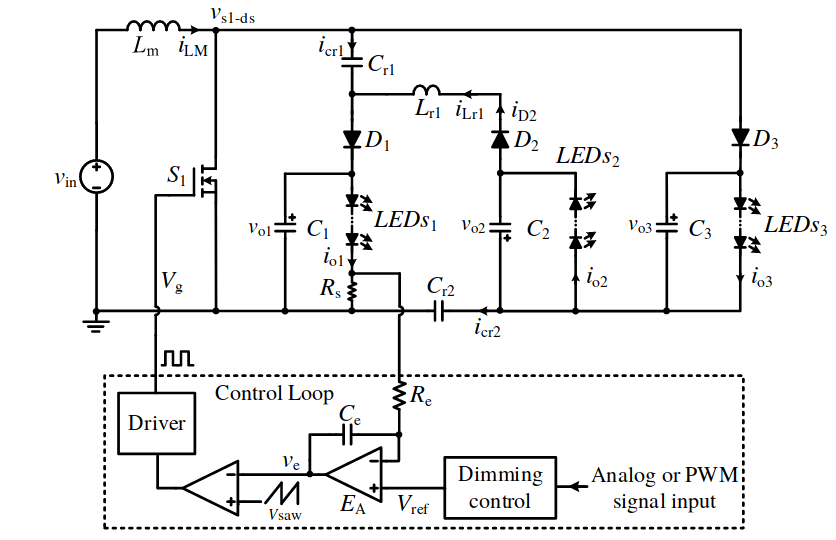
\includegraphics[scale = 0.42]{./fig/paper3}
    \caption{A bit more complex bucket converter.}
  \end{figure}	
\end{frame}

\begin{frame}{Circuit I designed}  
\begin{figure}
    \centering
    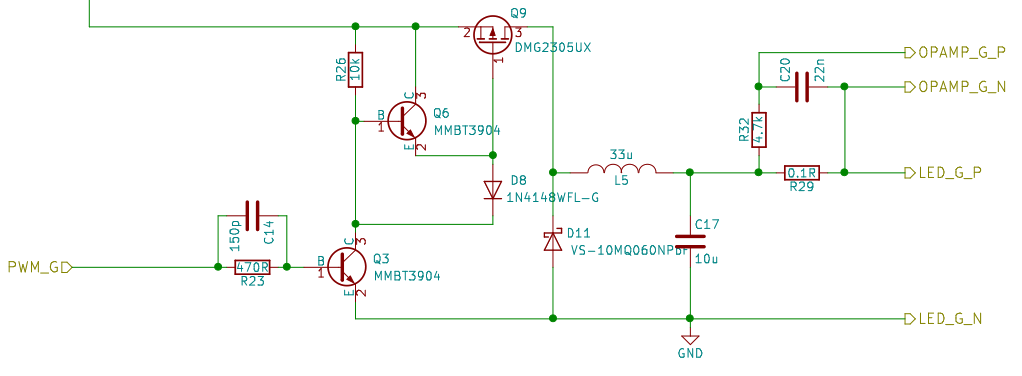
\includegraphics[scale = 0.42]{./fig/mycic}
    \caption{Quick gate charging bucket converter.}
  \end{figure}	
\end{frame}

\begin{frame}{THE PRINCIPLE OF REVERSED LAG APPLIED TO ON-OFF TEMPERATURE
CONTROL [H. SUTCLIFFE, 1960] (1)}
  \begin{figure}
    \centering
    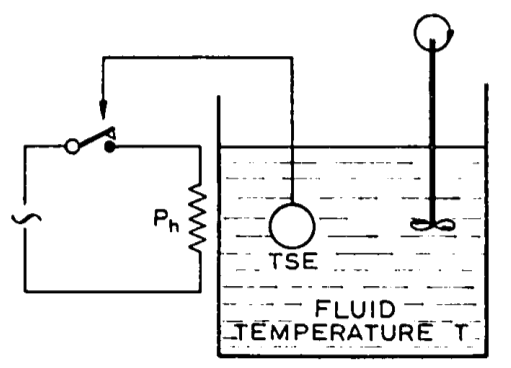
\includegraphics[scale = 0.6]{./fig/paper21}
    \caption{System overview of two-point control.}
  \end{figure}	
\end{frame}

\begin{frame}{THE PRINCIPLE OF REVERSED LAG APPLIED TO ON-OFF TEMPERATURE
CONTROL [H. SUTCLIFFE, 1960] (2)}
  \begin{figure}
    \centering
    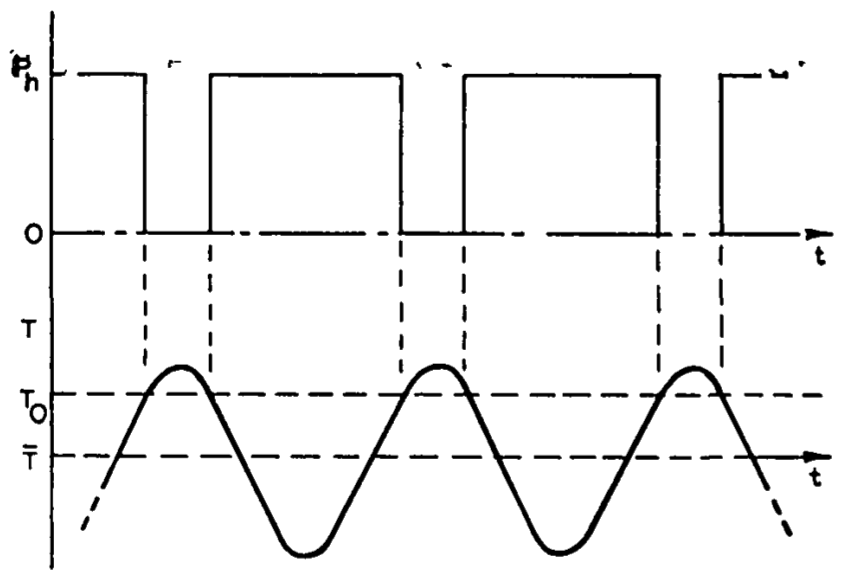
\includegraphics[scale = 0.4]{./fig/paper22}
    \caption{Low-pass behaviour of fluid being excited with a rectangular signal.}
  \end{figure}	
\end{frame}

\section{Market Analysis}

\begin{frame}{Target Group}
  \begin{itemize}
    \item<1-> Hackers
    \item<2-> Researchers, that want a quick prototype
    \item<3-> Engineers, that have no time to wait for China
    \item<4-> People, that watch videos like \href{https://www.youtube.com/watch?v=Hsw3lOnHaas}{this}

  \end{itemize}
 \end{frame}

\begin{frame}{Reichelt Elektronik}
  \centering
  \Huge www.reichelt.de
\end{frame}

\begin{frame}{Example of a modern Etching Machine from Reichelt}
\begin{figure}
    \centering
    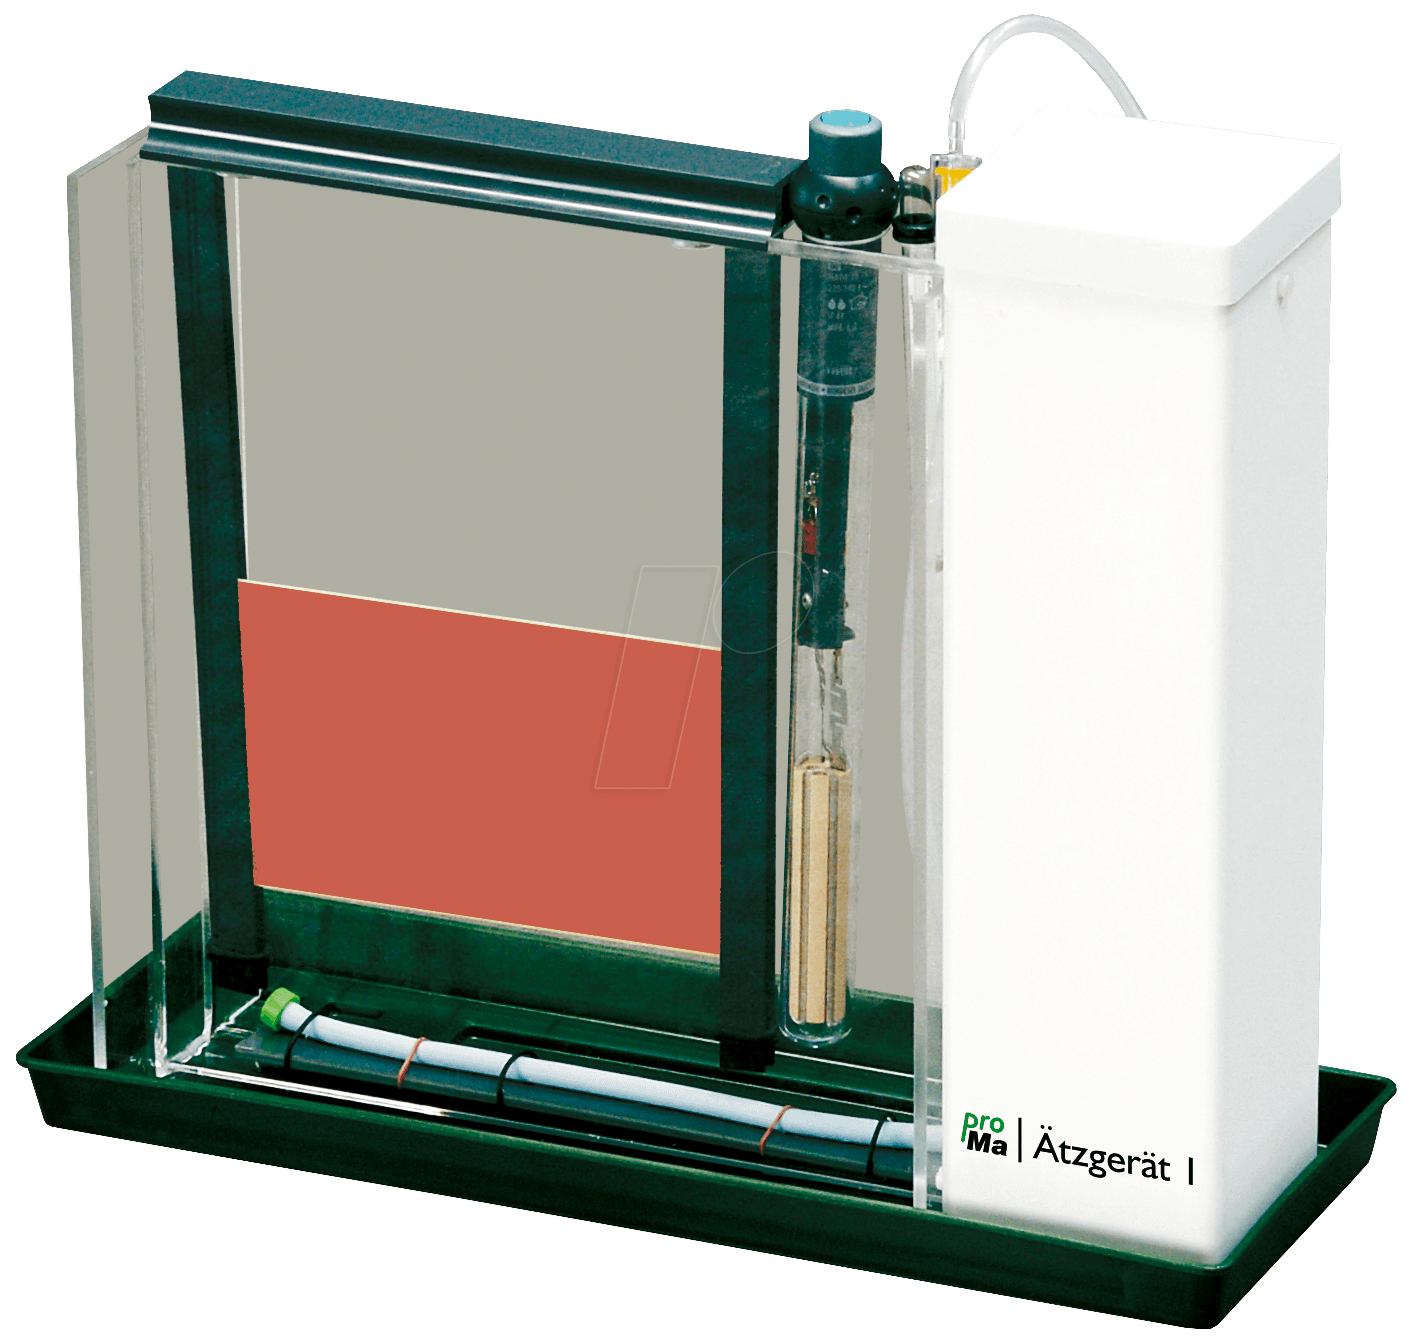
\includegraphics[scale = 0.13]{./fig/reichelt1}
    \caption{Price: 130 EUR. Needed Acid Volume: 1.75 l. Max. PCB Size: 235 mm x 170 mm. Heating Power: 100 W.}
  \end{figure}	
\end{frame}

\begin{frame}{Example of a modern UV Light from Reichelt}
\begin{figure}
    \centering
    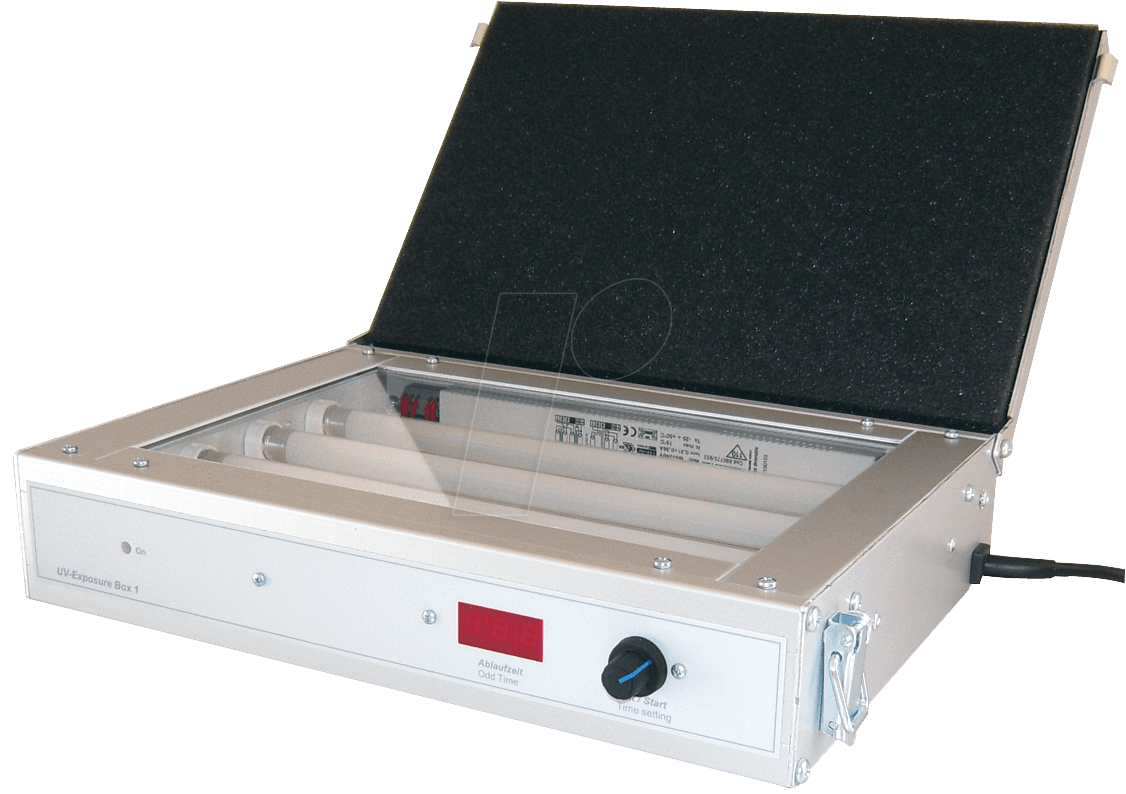
\includegraphics[scale = 0.2]{./fig/reichelt2}
    \caption{Price: 220 EUR. Max. PCB Size: 160 mm x 250 mm. Technology: Fluorescent Tubes (4 x 8 W). Weight: 4 kg.}
  \end{figure}	
\end{frame}

\begin{frame}{Our Goal}
  \begin{itemize}
    \item<1-> Build this equipment at home 
    \item<2-> Try to be cheaper and better
    \item<3> Provide a tutorial on how to build this equipment yourself
  \end{itemize}
\end{frame}

\begin{frame}[standout]
  Happy Coding :) 
\end{frame}

\end{document}
